\documentclass{article}
\usepackage[a4paper,landscape,margin=0cm]{geometry} % Zero margins for full-page design
\usepackage{graphicx} % For including images
\usepackage[x11names]{xcolor} % For color customization
\usepackage{tikz} % For advanced layout design
\usepackage{setspace}
% Set the path to your image directory
\graphicspath{{/home/blake/Documents/python/ChemLabelApp/}}

\begin{document}

% Start TikZ picture with overlay to use absolute positioning
\begin{tikzpicture}[remember picture, overlay]
    \def\inset{.25cm}    

    % Optional: Draw a grid for debugging (remove/comment out in final version)
    % \draw[step=1cm, gray, thin] (current page.north west) grid (current page.south east);

    % Draw a full-page border with rounded corners
    \draw[very thick, rounded corners=30pt] 
        ([shift={(\inset,-\inset)}]current page.north west) 
        rectangle 
        ([shift={(-\inset,\inset)}]current page.south east);

    % --- Images on the Top Right ---
    % QR Code
    \node[anchor=north east, 
          draw,
          rounded corners=15pt,
          very thick,
          inner sep=.25cm,
          text width = 6cm] 
        at ([xshift=-1cm, yshift=-.75cm]current page.north east) 
        {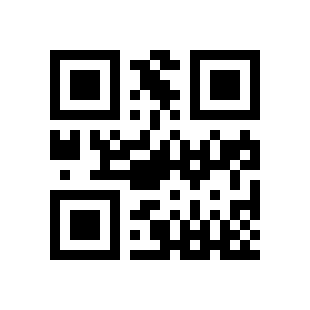
\includegraphics[width=6cm]{qr_code.png}};
    
    % Barcode
    \node[anchor=north east,
          draw,
          rounded corners=15pt,
          very thick,
          inner sep=.25cm,
          text width = 6cm] 
        at ([xshift=-8cm, yshift=-1.25cm]current page.north east) 
        {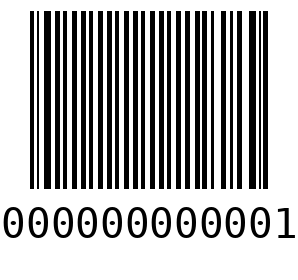
\includegraphics[width=6cm]{barcode.png}};

    % --- Image on the Top Left ---
    \node[anchor=north west,
          draw,                  % Draws the border
          rounded corners=15pt,  % Sets the radius of the rounded corners
          fill=black,          % Fills the box with a light blue color
          text width=8cm,        % Sets the width of the text area
          align=center,          % Centers the text
          font=\large]           % Sets the font size 
          at ([xshift=1cm, yshift=-1cm]current page.north west) 
        {
\includegraphics[width=8cm]{resources/images/sofab_logo.png}};

    % --- Product Details in the Middle Left ---
    \node[anchor=north west, align=left, font=\large] 
        at ([xshift=1cm, yshift=-4cm]current page.north west) 
    {
        {\LARGE \textbf{Product Name:} Amazing Product}\\[0.5cm]
        {\LARGE \textbf{SKU:} 12345}\\[0.5cm]
        {\LARGE \textbf{Weight:} 1kg}\\[0.5cm]
        {\LARGE \textbf{Manufacturer:} Example Corp} \\[0.5cm]
        {\LARGE \textbf{Usage Instructions:} Lorem ipsum dolor sit amet}
    };

    % --- Hazard Details on the Right/Bottom ---
    \node[anchor=south west, align=left,
        draw,                  % Draws the border
        rounded corners=15pt,  % Sets the radius of the rounded corners
        fill=Yellow1,          % Fills the box with a light blue color
        text width=7cm,        % Sets the width of the text area
        minimum height = 8cm,
        align=center,          % Centers the text
        font=\large]           % Sets the font size 
        at ([xshift=1cm, yshift=1.5cm]current page.south west) 
    {
        \textbf{Hazard Information:}\\[0.25cm]
        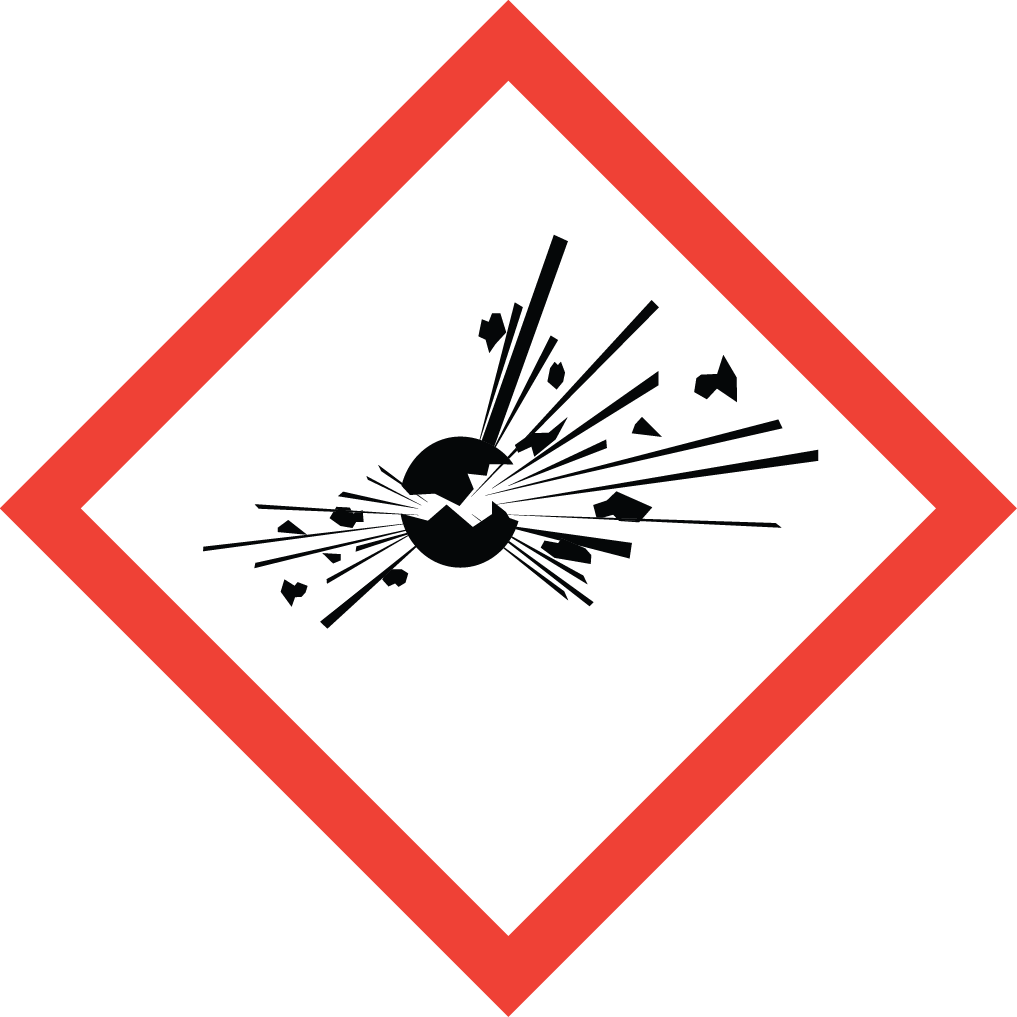
\includegraphics[width=2cm]{resources/images/hazard_diamonds/explosives.png} \quad 
        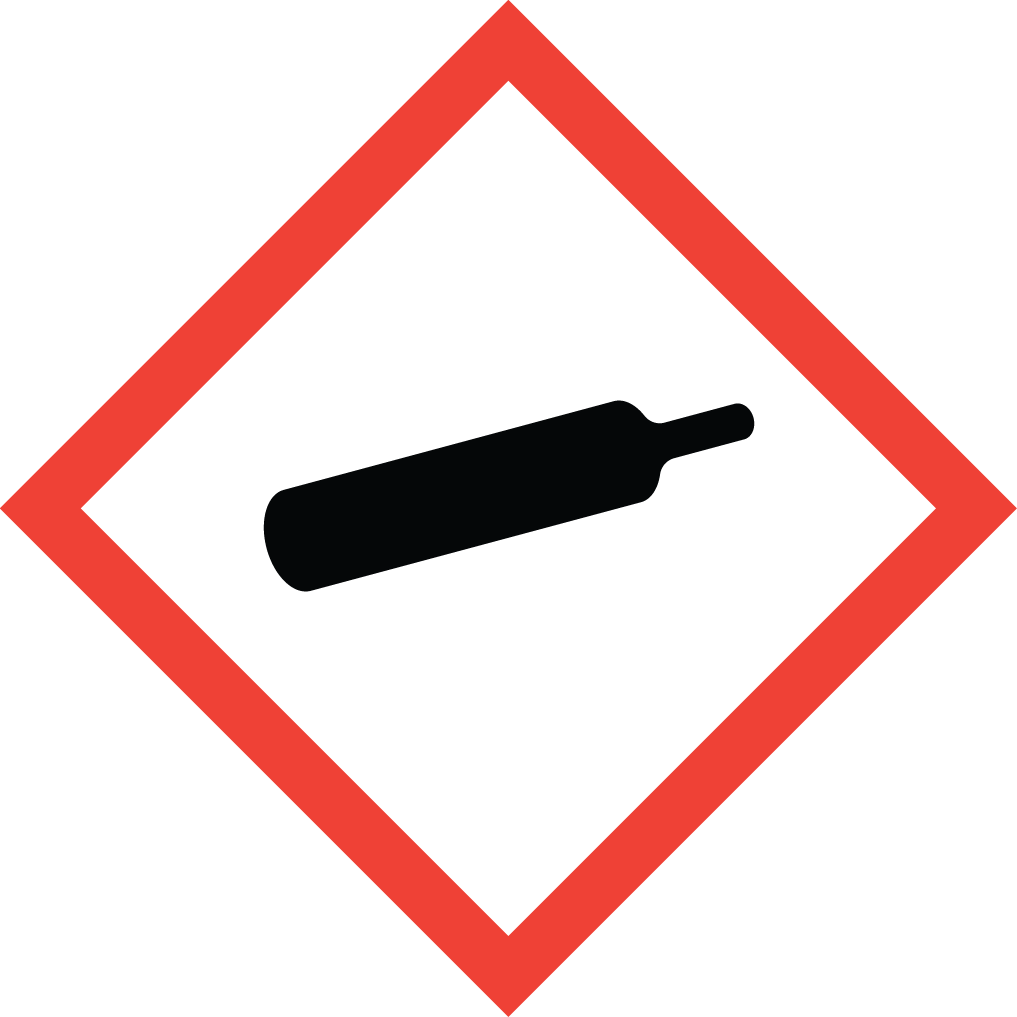
\includegraphics[width=2cm]{resources/images/hazard_diamonds/gasses.png}\\
    };

    % --- Hazard Details on the Right/Bottom ---
    \node[anchor=south west, align=left,
        draw,                  % Draws the border
        very thick,
        rounded corners=15pt,  % Sets the radius of the rounded corners
        fill=Red2,          % Fills the box with a light blue color
        text width=18cm,        % Sets the width of the text area
        minimum height = 8cm,
        align=center,          % Centers the text
        font=\large]           % Sets the font size 
        at ([xshift=10cm, yshift=1.5cm]current page.south west) 
    {
        \textbf{Warnings:}\\
        Keep away from children. Avoid contact with eyes.
    };
\end{tikzpicture}

\end{document}
